\chapter{Reproducción de algoritmos de PCL: Visualización de nubes y extracción de keypoints}

\section{Introducción}
Dejando asentado el fundamento teórico ofrecido por capítulos anteriores, se plantea a continuación la creación de dos programas de modo que, dada una nube de puntos, uno de ellos pueda visualizarla y otro extraiga keypoints.

Se cambia entonces la tonalidad del trabajo a partir del presente capítulo puesto que se trata de trabajo elaborado por el propio autor en vez de la constancia de investigación y explicaciones teóricas ya creadas y desarrolladas por terceros.

\section{Generación de programas a partir de código en C++}
La reproducción de los algoritmos de PCL está escrita en el mismo lenguaje que la propia librería, C++, a partir del cual hay que crear un ejecutable. Se parte de un directorio de trabajo llamado, por ejemplo, "prueba" en el que se encuentran:

\begin{itemize}
\item[•]prueba.cpp: Es el código escrito en C++ y que no tiene ninguna funcionalidad de por sí. 

\item[•]CMakeLists.txt: Es un fichero de texto utilizado para generar de forma automática un makefile y a partir de éste poder compilar el código fuente para conseguir un ejecutable. Un ejemplo de CMakeLists.txt es el siguiente:

\begin{lstlisting}
cmake_minimum_required(VERSION 2.6 FATAL_ERROR)	
project(PRUEBA)	
find_package(PCL 1.3 REQUIRED)	
include_directories(${PCL_INCLUDE_DIRS})	
link_directories(${PCL_LIBRARY_DIRS})	
add_definitions(${PCL_DEFINITIONS})	
add_executable(pcd_write_test pcd_write.cpp)	
target_link_libraries(pcd_write_test ${PCL_COMMON_LIBRARIES} ${PCL_IO_LIBRARIES})	
\end{lstlisting}

Donde se indica por orden: 

\begin{itemize}
\item[1]Mínima versión de cmake requerida
\item[2]Nombre del proyecto
\item[3]Búsqueda de librería PCL con versión mínima 1.3
\item[4]Inclusión de directorios de los encabezamientos de la librería PCL
\item[5]Inclusión de directorios de instalación de PCL y las librerías auxiliares
\item[6]Definiciones del preprocesador y banderas de compilación
\item[7]Nombre del ejecutable 
\item[8]Se indica al linker la librería de PCL
\end{itemize}

\item[•]build: Es una carpeta donde almacenar el ejecutable generado a partir del código fuente, el makefile y demás archivos necesarios para la compilación.
\end{itemize}

Una vez creados el código fuente, CMakeLists.txt y build, se ejecutan los siguientes comandos para generar el ejecutable:

$$cd \;\; build$$
$$sudo \;\; cmake \;\; ..$$
$$sudo \;\; make$$

Si todo sale bien, aparecerá un ejecutable en la carpeta build con el nombre indicado en CMakeLists.txt

Puesto que el código escrito en cualquier lenguaje de programación puede resultar complicado de transmitir, la forma de proceder para conseguir dicho objetivo será la siguiente; En primer lugar se explicará en alto nivel el programa en cuestión sin necesidad de leer código y haciendo uso de flujogramas u otros métodos que se consideren adecuados. Después, habiendo entendido la funcionalidad del programa, se pasará a explicar el código que lo compone con el nivel de detalle adecuado en cada momento. Para esto, también aparecerán flujogramas así como la explicación de las partes más importantes.

 
\section{Visualización de nubes de puntos}

Tal y como se ha mencionado en el apartado de objetivos del presente trabajo, la visualización de nubes se considera un hito transversal pero que a la vez involucra todo el proyecto ya que es la parte más amigable al ojo humano para estudiar resultados. De este modo se aprovecha el libre uso de la documentación y los tutoriales ofrecidos por PCL para modificar el código a favor de los objetivos planteados en el TFG.
%http://pointclouds.org/documentation/tutorials/

Se recuerda que la visualización de nubes no puede llevarse a cabo en la FPGA sobre la que se implementan los objetivos principales del trabajo ya que ésta no dispone de interfaz gráfica.

\subsubsection{Explicación en alto nivel}
Para la visualización de una nube de puntos con o sin sus puntos SIFT se necesita en primer lugar hacer uso del módulo IO que permite leer nubes en formato PCD. De esta forma se puede:

\begin{itemize}
\item[•]Leer una única nube de puntos para mostrarla por pantalla como tal.
\item[•]Leer dos nubes de puntos, en primer lugar una nube de puntos A y posteriormente una nube de puntos B que contiene los puntos SIFT de la nube A. De esta forma, se resaltan visualmente los puntos contenidos en la nube B y se visualiza junto a la nube A de modo que se pueden ver en conjunto todos los puntos de la nube original, tanto los que son keypoints como los que no. 
\end{itemize}

Cuando la nube está cargada, utilizando el módulo visualization, se crea una nueva ventana que hace de visualizador y en la que aparecen los tres ejes coordenados XYZ y el conjunto de puntos que conforman la nube situados en el espacio respecto al origen de los mencionados ejes. Cuando el usuario lo desee, puede cerrar la ventana que el programa ha creado para terminarlo.

Este conjunto de operaciones se muestran en su explicación en alto nivel en forma de flujograma en la figura \ref{fig:visualization_all_diagram}

\begin{figure}
\centering
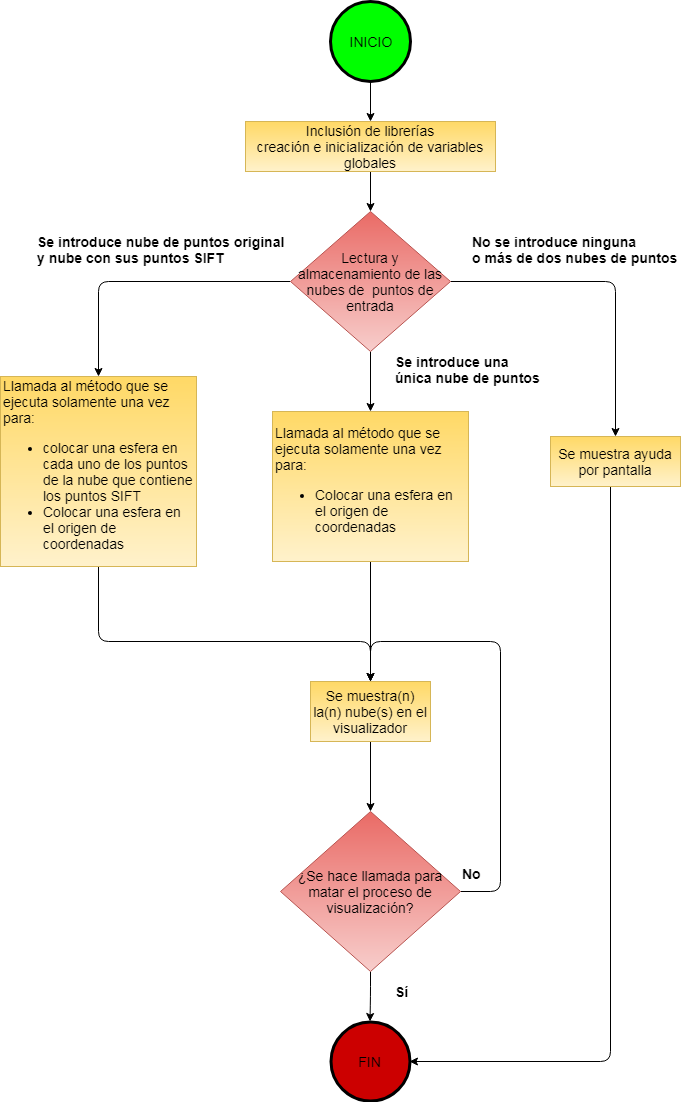
\includegraphics[scale=0.5]{visualization_all_diagram}
\caption{Flujograma del proceso de visualización de nubes de puntos.}\label{fig:visualization_all_diagram}
\end{figure}


\subsubsection{Explicación en bajo nivel}
El ejecutable generado dentro de la carpeta build se llama $visualization$ y para hacer funcionar el programa se han de ejecutar estos comandos, que en caso de querer visualizar una nube sin sus puntos SIFT:

$$./visualization \;\; nube1.pcd$$

y para visualizar una nube y sus keypoints:
$$./visualization \;\; nube1.pcd \;\; nube1\_keypoints.pcd$$

Véase a continuación el código que hace posible la funcionalidad ya explicada.\\

En primer lugar, se cargan las librerías de $iostream$ para las funcionalidades básicas de C++ y determinados módulos de la librería PCL; $IO$ para la lectura de nubes, $cloud\_viewer$ del módulo $visualization$ para la visualización de nubes y $parse$ del módulo $console$ para poder evaluar los argumentos introducidos por la consola de comandos.
Además, se crea la instancia $sift\_cloud$ de la clase $PointCloud$, es decir, una nube de puntos donde almacenar y modificar (resaltar puntos) la nube que contiene keypoints.

\begin{lstlisting}[language=C++,breaklines]
#include <iostream>
#include <pcl/visualization/cloud_viewer.h>
#include <pcl/io/io.h>
#include <pcl/io/pcd_io.h>
#include <pcl/console/parse.h>
pcl::PointCloud<pcl::PointXYZRGBA>::Ptr sift_cloud (new pcl::PointCloud<pcl::PointXYZRGBA>);
\end{lstlisting}

A continuación se implementa el método que muestra ayuda por pantalla.

\begin{lstlisting}[language=C++,breaklines]
void 
printUsage (const char* progName)
{
  std::cout << "\n\nUsage: "<<progName<<" <cloud.pcd> (optional <SIFTpoints.pcd>)\n\n";
}
\end{lstlisting}

En el siguiente fragmento de código se implementan las funciones que se ejecutan de forma excluyente una sola vez cuando se abre la ventana que visualiza la nube de puntos. 
Si se introduce una sola nube de puntos como entrada del programa, se ejecuta $viewerOneOff$ para añadir una esfera en el origen de coordenadas y así localizarlo fácilmente.
Por otra parte, si se introducen dos nubes de puntos, la original y la que contiene sus puntos SIFT, se ejecuta $viewerOneOffSIFT$ que hace lo mismo que la función anterior con el añadido de modificar la nube $sift\_cloud$ para añadir esferas en cada uno de sus puntos y distinguirlos de los de la nube original.
Además, se configura el color de fondo del visualizador aportando pesos a los valores máximos de color rojo, verde y azul que se pueden soportar; 1.0 para el color rojo y 0.5 para los colores verde y azul. 
El método $addSphere$ permite añadir al visualizador una esfera en el punto indicado.

\begin{lstlisting}[language=C++,breaklines]
void 
viewerOneOff (pcl::visualization::PCLVisualizer& viewer)
{
    viewer.setBackgroundColor (1.0, 0.5, 0.5);
    pcl::PointXYZ o;
    o.x = 0;
    o.y = 0;
    o.z = 0;
    viewer.addSphere (o, 0.01, "sphere", 0); 
}

void 
viewerOneOffSIFT (pcl::visualization::PCLVisualizer& viewer)
{
    viewer.setBackgroundColor (1.0, 0.5, 0.5);
    pcl::PointXYZ o;
    o.x = 0;
    o.y = 0;
    o.z = 0;
    viewer.addSphere (o, 0.01, "central sphere", 0);
    
    for(size_t i=0;i<sift_cloud->points.size();i++){
    	viewer.addSphere(sift_cloud->points[i],0.02f,50,255,50,std::to_string(i));	
    }
}
\end{lstlisting}

En el método principal $main$ se efectúa en primer lugar la comprobación del número de argumentos para ver si se han introducido una o dos nubes. En caso contrario se muestra ayuda por pantalla y se termina el programa.

\begin{lstlisting}[language=C++,breaklines]
int 
main (int argc, char** argv)
{   
    if(argc <= 1 || argc > 3 || (pcl::console::find_argument (argc,argv,"-h")) >= 0 )
    {
	printUsage (argv[0]);
	return 0;
    } 
\end{lstlisting}

Ahora se crea la instancia $cloud$ de la clase $PointCloud$ y se guarda en ella la nube original, se muestra por pantalla el número de puntos contenidos en la misma y se crea la instancia del visualizador llamada $viewer$

\begin{lstlisting}[language=C++,breaklines]
pcl::PointCloud<pcl::PointXYZRGBA>::Ptr cloud (new pcl::PointCloud<pcl::PointXYZRGBA>); 
    pcl::io::loadPCDFile(argv[1],*cloud);
    cout << "\nNumber of points in input cloud: " << cloud->points.size() << "\n";

    pcl::visualization::CloudViewer viewer("Cloud Viewer");
\end{lstlisting}

Si se ha introducido una nube como argumento se asigna al visualizador la función $viewerOneOff$ para ejecutarse una vez al inicio de la visualización y posteriormente se muestra la nube.

\begin{lstlisting}[language=C++,breaklines]
if (argc == 2)
    {
	viewer.runOnVisualizationThreadOnce (viewerOneOff);
	viewer.showCloud(cloud,"cloud");
    }
\end{lstlisting}

Si se introducen dos nubes se carga la segunda en la instancia $sift\_cloud$, se asigna la función $viewerOneOffSIFT$ al visualizador y se muestran las dos nubes en el mismo.

\begin{lstlisting}[language=C++,breaklines]
else 
    {
	pcl::io::loadPCDFile(argv[2],*sift_cloud);
        cout << "\nNumber of points in SIFT cloud: " << sift_cloud->points.size() << "\n";

viewer.runOnVisualizationThreadOnce (viewerOneOffSIFT);
    	viewer.showCloud(cloud,"cloud");
   	viewer.showCloud(sift_cloud,"sift_cloud");
 
    }
\end{lstlisting}

Por último, el bloqueo del programa en el visualizador hasta que el usuario lo detiene.
\begin{lstlisting}[language=C++,breaklines]
   while (!viewer.wasStopped ())
    {
    }
    return 0;
}
\end{lstlisting}

\section{Programa principal: Extracción de puntos SIFT}
\subsubsection{Explicación en alto nivel}
Se muestra en la figura \ref{fig:main_HL_diagram} el flujograma que representa el funcionamiento del programa principal capaz de extraer puntos SIFT dada una nube de puntos como entrada. Se aprecia que hay dos operaciones principales; extracción de normales y extracción de puntos SIFT. Más adelante se estudiarán los tiempos necesarios para efectuar cada una de las operaciones y se decidirá cuál es la de mayor carga computacional y por tanto cuál hay que optimizar.

\begin{figure}
\centering
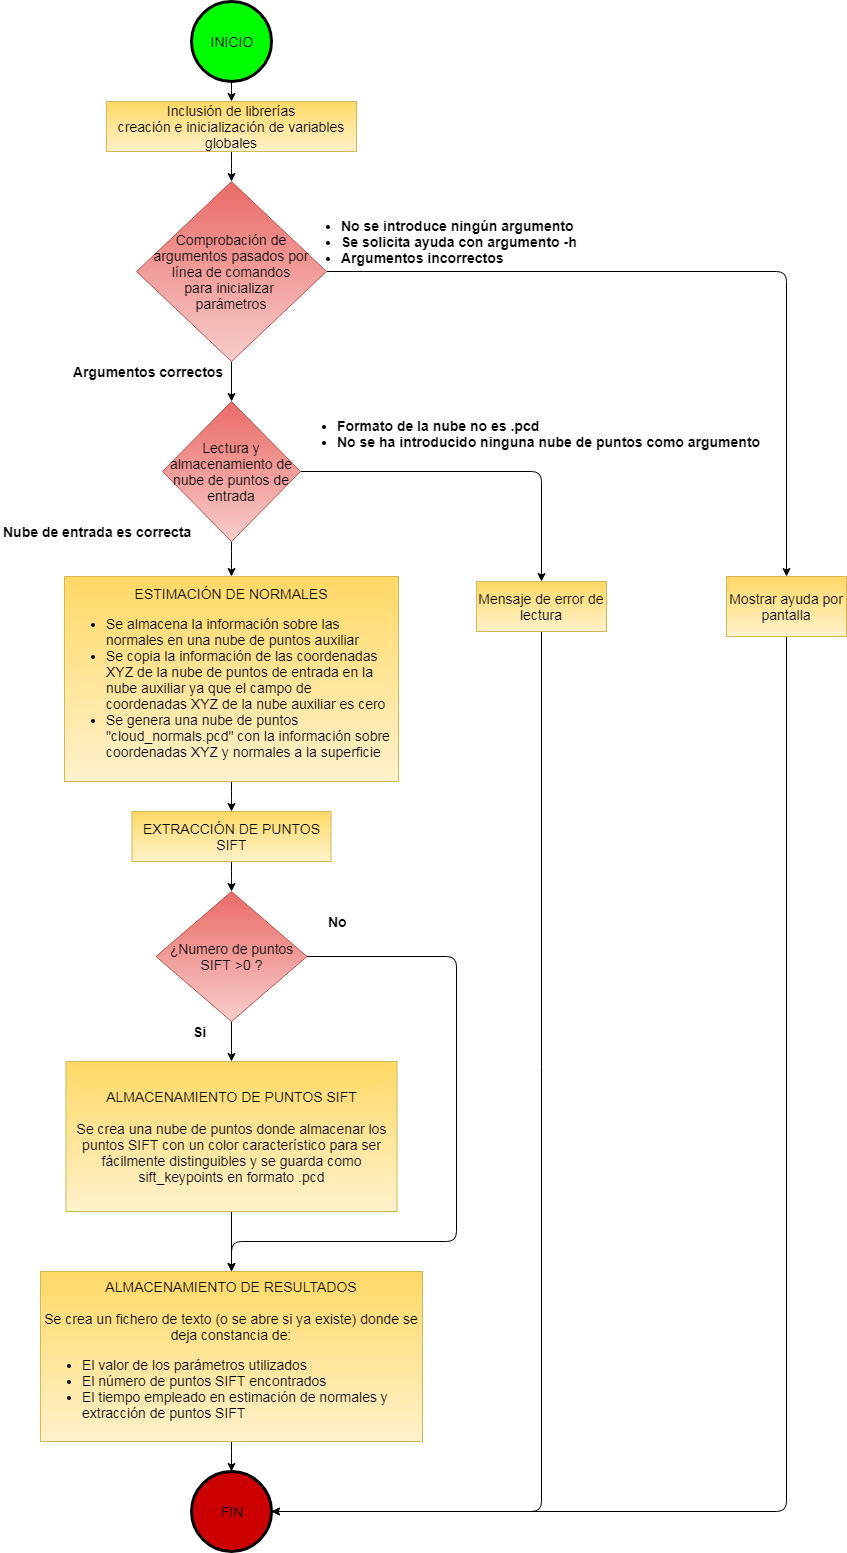
\includegraphics[scale=0.45]{main_HL_diagram}
\caption{Flujograma que representa el proceso de extracción de puntos SIFT.}\label{fig:main_HL_diagram}
\end{figure}

\subsubsection{Explicación en bajo nivel}
Antes de entrar en detalle en el código que compone este programa, se indica la forma de hacer uso del mismo. 
El nombre del ejecutable para este programa es $sift\_keypoints$ al cual se llama con dos tipos de argumentos; parámetros y nube de puntos. Los primeros son opcionales ya que tienen valores por defecto pero el segundo es obligatorio. El esquema de llamada al ejecutable es el siguiente:

$$sudo \;\; ./sift\_keypoints \;\; -parametro1 \;\; valor1 \;\; -parametro2 \;\; valor2 \;\; ... \;\; -parametroN \;\; valorN \;\; nube.pcd$$

Se requieren permisos de super usuario debido a operaciones de escritura tal y como son modificar y guardar un fichero de texto o guardar nubes de puntos en formato PCD.


Estudiando el código de este programa, en primer lugar se incluyen la librería iostream y los módulos necesarios de la librería de PCL. No se muestra esta parte del código ya que es trivial y muy semejante al ya mostrado en el programa de visualización.

A continuación se crean e inicializan el conjunto de variables globales necesarias cuyo significado se explicará según se requiera su uso a lo largo del programa. Como excepción se tienen las variables $begin$, $end$, $elapsed\_sec$, $normal\_estimation\_time$ y $sift\_estimation\_time$ que sirven para medir tiempos de ejecución por lo que entrarán en juego en el siguiente capítulo.

\begin{lstlisting}[language=C++,breaklines]
int normal_estimation_object = 0;
float radius_search = 0.02f;
float normal_estimation_time = 0.0f;
float sift_estimation_time = 0.0f;

float min_scale = 0.01f;
int n_octaves = 3;
int n_scales_per_octave = 4;
float min_contrast = 0.001f;
int sift_points=0; 

clock_t begin,end;
double elapsed_sec;
\end{lstlisting}


Se implementa ahora el método que muestra ayuda por pantalla que informa sobre cómo utilizar el programa y los posibles parámetros que acepta.

\begin{lstlisting}[language=C++,breaklines]
void 
printUsage (const char* progName)
{
  std::cout << "\n\nUsage: "<<progName<<" [options] <scene.pcd>\n\n"
            << "Options:\n"
            << "-------------------------------------------\n"
            << "-o <integer>	0 for regular normal estimation (default), 1 for enhanced normal estimation\n"
            << "-r <float>	Radius search for normal estimation (default "<< radius_search<<")\n"
            << "-ms <float>	Minimum scale (default " << min_scale << ")\n"
            << "-no <int>	Number of octaves (default " << n_octaves << ")\n"
            << "-ns <int>	Number of scales per octave (default " << n_scales_per_octave << ")\n"
	    	<< "-mc <float>	Minimum contrast (default " << min_contrast << ")\n"
	    	<< "-h		Show help\n"
            << "\n\n";
}
\end{lstlisting}


A continuación, se implementa el método principal "main" y que ocupa el resto del código.\\
Primeramente, se comprueba si el número de argumentos es el correcto o se ha pedido ayuda con el argumento $-h$ y se muestran por pantalla el valor de los parámetros, ya sea el establecido con argumentos por línea de comandos o sus valores por defecto.
Además, se crea la instancia $ne$ de la clase $NormalEstimation$ o $NormalEstimationOMP$ según el valor del parámetro correspondiente pasado por línea de comandos. La clase $NormalEstimation$ sirve para la estimación estándar de normales mientras que $NormalEstimationOMP$ permite realizar esta misma operación entre 6 y 8 veces más rápido para equipos con procesadores de 8 núcleos (queda excluida la FPGA usada en el presente trabajo). Esta clase es compatible con la estándar pero solamente se aprecian mejoras sustanciales en tiempo de computación si se dispone de un equipo suficientemente potente.

%http://pointclouds.org/documentation/tutorials/normal_estimation.php

\begin{lstlisting}[language=C++,breaklines]
int main(int argc, char** argv)
{
  if(argc == 1 || (pcl::console::find_argument (argc,argv,"-h") >= 0) )
  {
	printUsage (argv[0]);
	return 0;
  }	

  std::cout << std::endl << "---Normal estimation parameters---" << std::endl;

  pcl::NormalEstimation<pcl::PointXYZ, pcl::PointNormal> ne;
  pcl::console::parse (argc, argv, "-o", normal_estimation_object);
  if(normal_estimation_object >0)
  {
	std::cout << "Using enhanced normal estimation object" << std::endl;
	pcl::NormalEstimationOMP<pcl::PointXYZ, pcl::PointNormal> ne;
  }
  else
  {
	std::cout << "Using regular normal estimation object" << std::endl;
  }
  
  pcl::console::parse (argc,argv, "-r", radius_search);
  std::cout << "Setting radius search for normal estimation to: " << radius_search << std::endl;

  
  std::cout << std::endl << "---Sift points parameters---" << std::endl;
  
  
  pcl::console::parse (argc,argv, "-ms", min_scale);
  std::cout << "Setting minimum scale to: " << min_scale << std::endl;

  pcl::console::parse (argc,argv, "-no", n_octaves);
  std::cout << "Setting number of octaves to: " << n_octaves << std::endl;

  pcl::console::parse (argc,argv, "-ns", n_scales_per_octave);
  std::cout << "Setting number of scales per octave to: " << n_scales_per_octave << std::endl;

  pcl::console::parse (argc,argv, "-mc", min_contrast);
  std::cout << "Setting minimum contrast to: " << min_contrast << std::endl;

  std::cout << std::endl << std::endl;
\end{lstlisting}

Ahora se efectúa la lectura de la nube de puntos comprobando que se ha introducido como argumento un archivo en formato PCD y que éste puede leerse. La nube se almacena en $cloud\_xyz$ que es una instancia de la clase $PointCloud$.

\begin{lstlisting}[language=C++,breaklines]
  begin = clock();

  pcl::PointCloud<pcl::PointXYZ>::Ptr cloud_xyz (new pcl::PointCloud<pcl::PointXYZ>);
  std::vector<int> pcd_filename_indices = pcl::console::parse_file_extension_argument (argc, argv, "pcd"); 
  std::string filename;
     
  std::cout << "Reading file..." << std::endl;

  if (!pcd_filename_indices.empty ())
  {
  	filename = argv[pcd_filename_indices[0]];
  	if (pcl::io::loadPCDFile (filename, *cloud_xyz) == -1) 
    	{
        	std::cout << "Was not able to open file \""<<filename<<"\".\n";
       		return -1;
    	}
  }
  else
  {
  	std::cout << "\nNo *.pcd file given => closing.\n\n";
  	return -1;
  }
  
  end = clock();
  elapsed_sec = double(end-begin)/CLOCKS_PER_SEC;
  std::cout << "Number of points in "<< filename << ": "<< cloud_xyz->points.size () <<std::endl; 
  std::cout << "Time needed for " << filename << " to load: " << elapsed_sec << " seconds"<< std::endl << std::endl; 
\end{lstlisting}
  
  
La siguiente parte del código se encarga de la extracción de normales en la superficie de la nube. Para ello se crea una instancia de la clase $PointCloud$ llamada $cloud\_normals$ y que va a almacenar una nube de puntos idéntica a la de entrada pero con información adicional sobre los vectores normales.
Retomando la instancia "ne" de la clase $NormalEstimation$, se llama al método $setInputCloud$ para asignar a esta instancia la nube de puntos con la que va a trabajar, es decir, $cloud\_xyz$, para que extraiga de ella los vectores normales.
Además, entran en juego un par de parámetros que se asignan con los métodos $setSearchMethod$ y $setRadiusSearch$ y sirven para establecer respectivamente el método de búsqueda de normales y el radio de la esfera (en centímetros) dentro de la que buscar normales, siendo el centro de la misma cada punto de la nube en cada iteración.
El método de búsqueda de normales se establece usando la instancia $tree\_n$ de la clase $KdTree$ y hace referencia a la partición o clasificación jerárquica del espacio en forma de árbol para agilizar las operaciones sobre la nube $cloud\_xyz$.
Una vez que todos los parámetros están asignados, se llama al método compute indicando que es la nube $cloud\_normals$ en la que hay que almacenar la información de los vectores normales extraídos de $cloud\_xyz$.

\begin{lstlisting}[language=C++,breaklines]
  pcl::PointCloud<pcl::PointNormal>::Ptr cloud_normals (new 		pcl::PointCloud<pcl::PointNormal>);
  pcl::search::KdTree<pcl::PointXYZ>::Ptr tree_n(new pcl::search::KdTree<pcl::PointXYZ>());

  ne.setInputCloud(cloud_xyz);
  ne.setSearchMethod(tree_n);
  ne.setRadiusSearch(radius_search);
 
  std::cout << "Estimating normals in " << filename << " surface..." <<std::endl;

  begin = clock();
  ne.compute(*cloud_normals);
  end = clock();

  normal_estimation_time = double(end-begin)/CLOCKS_PER_SEC;
  std::cout << "Time needed for normal estimation (compute) in " << filename << ": " << normal_estimation_time << " seconds" << std::endl << std::endl;
\end{lstlisting}
  
Debido a que el método compute solamente guarda en $cloud\_normals$ los vectores normales extraídos de la nube $cloud\_xyz$, la primera carece de información de coordenadas XYZ sobre los puntos originales. Por lo tanto, se copia dicha información de $cloud\_xyz$ a $cloud\_normals$.

\begin{lstlisting}[language=C++,breaklines]
  std::cout << "Copying xyz information from" << filename << " to cloud with normals information..." << std::endl;

  begin = clock();

  for(size_t i = 0; i<cloud_normals->points.size(); ++i)
  {
  	cloud_normals->points[i].x = cloud_xyz->points[i].x;
  	cloud_normals->points[i].y = cloud_xyz->points[i].y;
  	cloud_normals->points[i].z = cloud_xyz->points[i].z;
  }

  end = clock();
  elapsed_sec = double(end-begin)/CLOCKS_PER_SEC;
  std::cout << "Time needed for copying the pointcloud: " << elapsed_sec <<" seconds" << std::endl << std::endl;
\end{lstlisting}

  Si la nube $cloud\_normals$ no está vacía, se guarda en formato PCD bajo el nombre $cloud\_normals.pcd$
  
\begin{lstlisting}[language=C++,breaklines]
  if(cloud_normals->points.size()!=0){
  	pcl::io::savePCDFileASCII ("cloud_normals.pcd", *cloud_normals);
  }
\end{lstlisting}

El siguiente bloque de código hace referencia a la extracción de puntos SIFT creando en primer lugar la instancia $sift$ de la clase $SIFTKeypoint$, es decir, un punto del tipo SIFT sobre el cual se efectúan las operaciones pertinentes. Además, el resultado de la extracción, la nube con los puntos SIFT, se almacena en la instancia $result$ de la clase $PointCloud$

Aquí entran en juego más parámetros que en la extracción de normales:

Como ya se ha indicado antes, se crea una instancia $tree$ de la clase $KdTree$ para la labor de partición y organización jerárquica del espacio en forma de árbol y se asigna a $sift$ mediante el método $setSearchMethod$.
El método $setScales$ se encarga de asignar a $sift$ los parámetros $min\_scale$, $n\_octaves$ y $n\_scales\_per\_octave$ del tipo $float$, $int$ e $int$ respectivamente. Su significado es el siguiente:

\begin{itemize}
\item[•]$min\_scale$: Es la desviación estándar de la función Gaussiana para el primer desenfoque aplicado a la nube.
\item[•]$n\_octaves$: Número de octavas o conjunto de nubes del mismo tamaño a las que se les aplica diferentes desenfoques.
\item[•]$n\_scales\_per\_octave$: Es el número de desenfoques por octava.
\end{itemize}

Para comprender estos parámetros, hay que tener en cuenta que el algoritmo de extracción de puntos SIFT crea un espacio escalado a partir de la nube con la que trabaja. Esto se debe a que trata de reproducir la naturaleza "multiescala" de los objetos, es decir, los detalles que se aprecian de un árbol, por ejemplo, varían según la distancia a la que se encuentra el observador; A cincuenta metros de distancia se precia la forma, tamaño y colores principales del árbol mientras que a un metro de distancia se pueden ver otros detalles como la rugosidad del tronco o forma de las hojas. Además, dependiendo del observador, el nivel de los detalles detectados en el árbol varían.

Considerando una nube de puntos en dos dimensiones como una imagen plana, para construir un espacio escalado en primer lugar se toma la nube de puntos original con la función que la describe: 
$$f(x,y)$$ 

junto a la función Gaussiana:
$$G(x,y,\sigma)=\frac{1}{2\pi\sigma^2}e^{-\frac{x^2+y^2}{2\sigma^2}}$$

y se difumina, es decir, se hace una convolución: 
$$L(\cdot,\cdot,\sigma)=G(\cdot,\cdot,\sigma)*f(\cdot,\cdot)$$

La convolución se aplica para cada valor $x$ e $y$ siendo así el parámetro principal de la función Gaussiana la desviación típica que se indica con $min\_scale$. Esta operación se repite un número de veces indicado por el parámetro $n\_scales\_per\_octave$ e incrementando en cada iteración el valor de la desviación típica indicada en $min\_scale$ y por tanto el nivel de desenfoque.

Cuando se alcanza el número máximo de iteraciones, se toma la nube a la que se le ha aplicado el desenfoque con el mayor valor de la desviación típica y se reduce su tamaño a la mitad. Una vez hecho esto, se repite el proceso anterior para difuminar la nube mediante la función Gaussiana e incrementando su valor de la desviación típica. 

El proceso de reducción del tamaño de la nube para aplicar la convolución con la función Gaussiana se repite un número de veces indicado por el parámetro $n\_octaves$, es decir, número de octavas, ya que el tamaño de la nube se reduce a la mitad.

El proceso de creación del espacio escalado se puede visualizar en el ejemplo de la figura \ref{fig:filtro_gauss}. El propósito de este conjunto de operaciones es el de simular diferentes escalas de observación (movimiento vertical en la figura \ref{fig:filtro_gauss}) así como la apreciación de diferentes niveles de detalle en cada escala (movimiento horizontal en la figura \ref{fig:filtro_gauss})  

\begin{figure}
\centering
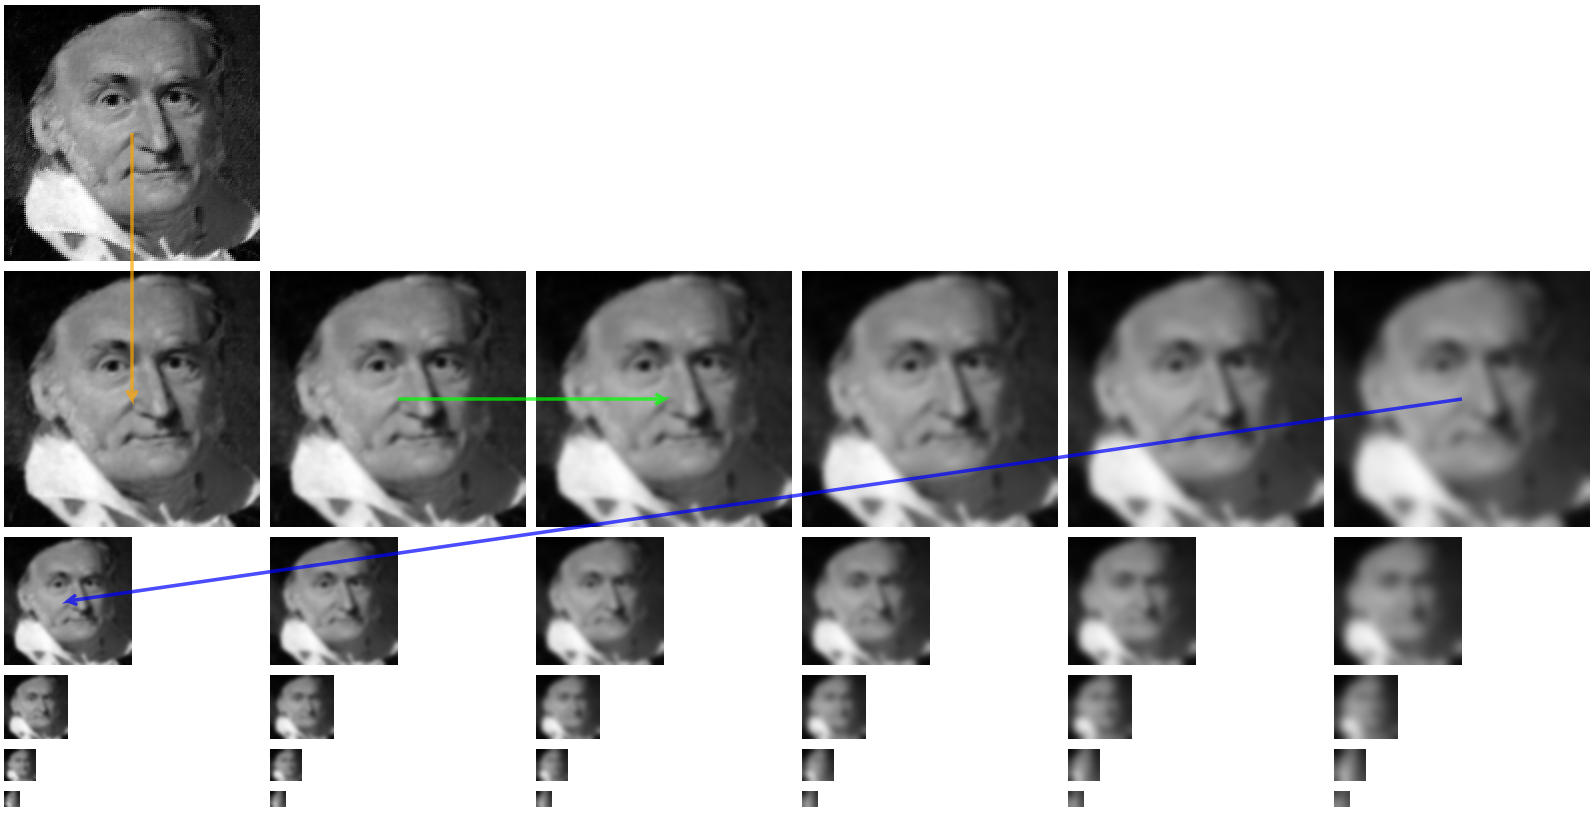
\includegraphics[scale=0.42]{filtro_gauss}
\caption{Ejemplo de creación de un espacio escalado. La flecha naranja indica el primer desenfoque aplicado a la imagen original. La flecha verde indica la convolución de la imagen con la función Gaussiana para desviaciones típicas crecientes. La flecha azul indica la creación de una nueva octava.}\label{fig:filtro_gauss}
\end{figure}



%https://en.wikipedia.org/wiki/Scale_space
%http://aishack.in/tutorials/sift-scale-invariant-feature-transform-scale-space/
%http://weitz.de/sift/
%http://aishack.in/tutorials/harris-corner-detector/

El último parámetro es $min\_contrast$ y se asigna a $sift$ con $setMinimumContrast$. Este parámetro actúa como un filtro para eliminar los puntos SIFT que no tienen suficiente contraste. Esto se consigue calculando dos gradientes perpendiculares en cada keypoint detectado de forma que la superficie entorno al keypoint puede ser plana (ambos gradientes tienen un valor pequeño), representar un borde (un gradiente tiene un valor elevado y el otro no) o representar una esquina (ambos gradientes toman valores significativos). Poner este parámetro a cero significa aceptar todos los keypoints detectados mientras que incrementarlo aumenta la dureza de la criba y por tanto la exigencia de contraste en cada uno de ellos.

Con $setInputCloud$ se asigna a $sift$ la nube con la que se trabaja que en el caso es $cloud\_normals$ y con $compute$ se efectúa la operación de extracción de puntos SIFT para almacenarlos en $result$.

%http://aishack.in/tutorials/harris-corner-detector/

\begin{lstlisting}[language=C++,breaklines]
  pcl::SIFTKeypoint<pcl::PointNormal, pcl::PointWithScale> sift;
  pcl::PointCloud<pcl::PointWithScale>::Ptr result(new pcl::PointCloud<pcl::PointWithScale>);
  pcl::search::KdTree<pcl::PointNormal>::Ptr tree(new pcl::search::KdTree<pcl::PointNormal> ());
  sift.setSearchMethod(tree);
  sift.setScales(min_scale, n_octaves, n_scales_per_octave);
  sift.setMinimumContrast(min_contrast);
  sift.setInputCloud(cloud_normals);
 
  std::cout << "Estimating sift points in " << filename << "..." << std::endl;

  begin = clock();
  sift.compute(*result);
  end = clock();
  sift_estimation_time = double(end-begin)/CLOCKS_PER_SEC;
  std::cout << "Time needed for sift point extraction: " << sift_estimation_time << " seconds" << std::endl << std::endl;
\end{lstlisting}

Si la nube $result$ no está vacía, es decir, se han encontrado puntos SIFT, se crea una instancia de una nueva nube llamada $keypoints$ y en ella se almacenan los puntos SIFT encontrados con información adicional sobre su color pues ahora serán verdes para su fácil visualización. Después, se guarda la nube $keypoints$ en formato PCD bajo el nombre $sift\_keypoints.pcd$
Esta nube de puntos junto a la nube de la que procede y de la cual se han extraído los keypoints, son las que se utilizan en el visualizador par apreciar una nube de puntos con sus keypoints resaltados.

\begin{lstlisting}[language=C++,breaklines]
  if(result->points.size()>0){
  
  	std::cout << "Number of SIFT points in " << filename << ": " << result->points.size () << std::endl;

	sift_points = result->points.size();

	pcl::PointCloud<pcl::PointXYZRGBA>::Ptr keypoints(new pcl::PointCloud<pcl::PointXYZRGBA>);
  
	keypoints->width = result->width;
	keypoints->height = result->height;
	keypoints->points.resize(keypoints->width * keypoints->height);

   	for (size_t i = 0; i < result->points.size (); ++i)
  	{
    	keypoints->points[i].x = result->points[i].x;
    	keypoints->points[i].y = result->points[i].y;
    	keypoints->points[i].z = result->points[i].z;

  		keypoints->points[i].r=50;
  		keypoints->points[i].g=255;
  		keypoints->points[i].b=50;
  		keypoints->points[i].a=255;
  	}
  	pcl::io::savePCDFileASCII ("sift_keypoints.pcd", *keypoints);
  }
  else {
  	std::cout << "No sift points found" << std::endl;
	sift_points = 0;
  }
\end{lstlisting}

 Por último, se abre o crea un fichero de texto llamado $tests.txt$ en el que se indica el nombre de la nube de puntos de entrada y el número de puntos que contiene, el valor de los parámetros utilizados en todas las operaciones que los requieren y el número de puntos SIFT encontrados.
 
\begin{lstlisting}[language=C++,breaklines]
  std::fstream fs;
  fs.open("tests.txt", std::fstream::app);
  
  fs << "filename: " << filename << std::endl;
  
  fs << std::endl <<  "Normal estimation radius search: " << radius_search << std::endl; 
  fs << "Minimum scale: " << min_scale << std::endl;
  fs << "Number of octaves: " << n_octaves << std::endl;
  fs << "Number of scales per octave: " << n_scales_per_octave << std::endl;
  fs << "Minimum contrast: " << min_contrast << std::endl;

  fs << std::endl << "Normal estimation time (s): " << normal_estimation_time << std::endl;
  fs << "SIFT points estimation time (s): " << sift_estimation_time << std::endl;
  fs << "Number of SIFT points found: " << sift_points << std::endl;

  fs << "---------------------\n----------------------\n";
  fs.close();
  return 0;
}
\end{lstlisting}


\section{Ejemplos de visualización y extracción de puntos SIFT}
Los siguientes ejemplos se han llevado a cabo en una computadora que dispone de máquina virtual con sistema operativo basado en linux. Todos ellos son reproducibles en la FPGA salvo los de visualización como ya se ha indicado previamente.

Se van a tomar como ejemplos tres nubes de puntos:
\begin{itemize}
\item[•]$bunny.pcd$: 
Con un total de 397 puntos representa un conejo. El encabezamiento del archivo es el siguiente:\\
\begin{lstlisting}
#bunny.pcd
#.PCD v.5 - Point Cloud Data file format
VERSION .5
FIELDS x y z
SIZE 4 4 4
TYPE F F F
COUNT 1 1 1
WIDTH 397
HEIGHT 1
POINTS 397
DATA ascii
\end{lstlisting}

\item[•]$cturtle.pcd$:
Contiene 167198 puntos que representan el caparazón de una tortuga. El encabezamiento del archivo se muestra a continuación:\\
\begin{lstlisting}
#cturtle.pcd
#.PCD v0.7 - Point Cloud Data file format
VERSION 0.7
FIELDS x y z intensity
SIZE 4 4 4 4
TYPE F F F F
COUNT 1 1 1 1
WIDTH 167198
HEIGHT 1
VIEWPOINT 0 0 0 1 0 0 0
POINTS 167198
DATA binary_compressed
\end{lstlisting}


\item[•]$milk\_cartoon\_all\_small\_clorox.pcd$:
Representa tres botes sobre una superficie mediante 307200 puntos. Su encabezamiento indica que es una nube ordenada, es decir, tiene una estructura matricial tal y como se indicó en la explicación del formato PCD.\\
\begin{lstlisting}
#milk_cartoon_all_small_clorox.pcd
#.PCD v0.7 - Point Cloud Data file format
VERSION 0.7
FIELDS x y z rgba
SIZE 4 4 4 4
TYPE F F F U
COUNT 1 1 1 1
WIDTH 640
HEIGHT 480
VIEWPOINT 0 0 0 1 0 0 0
POINTS 307200
DATA binary_compressed
\end{lstlisting}

\end{itemize}

Se puede apreciar en los encabezamientos de las nubes que el tipo de datos en $bunny.pcd$ es $ascii$ mientras que en las otras dos nubes es $binary\_compressed$. Esto se debe a la gran cantidad de puntos que contienen por lo que el formato $ascii$ se comprime en $binary\_compressed$ para que el archivo ocupe menos espacio.

\subsection{Visualización}
Para visualizar estas nubes se ejecutan los siguientes comandos pudiendo ver los resultados en las figuras \ref{fig:bunny_ejemplo}, \ref{fig:cturtle_ejemplo} y \ref{fig:botes} 
$$./visualization\;\;bunny.pcd$$
$$./visualization\;\;cturtle.pcd$$
$$./visualization\;\;milk\_cartoon\_all\_small\_clorox.pcd$$

\begin{figure}[!htb]
\minipage{0.32\textwidth}
  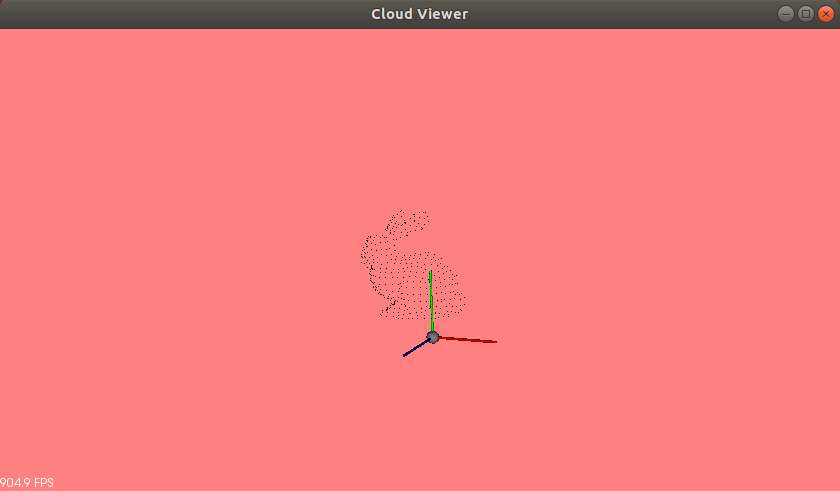
\includegraphics[width=\linewidth]{bunny_ejemplo}
  \caption{Visualización de la nube $bunny.pcd$}\label{fig:bunny_ejemplo}
\endminipage\hfill
\minipage{0.32\textwidth}
  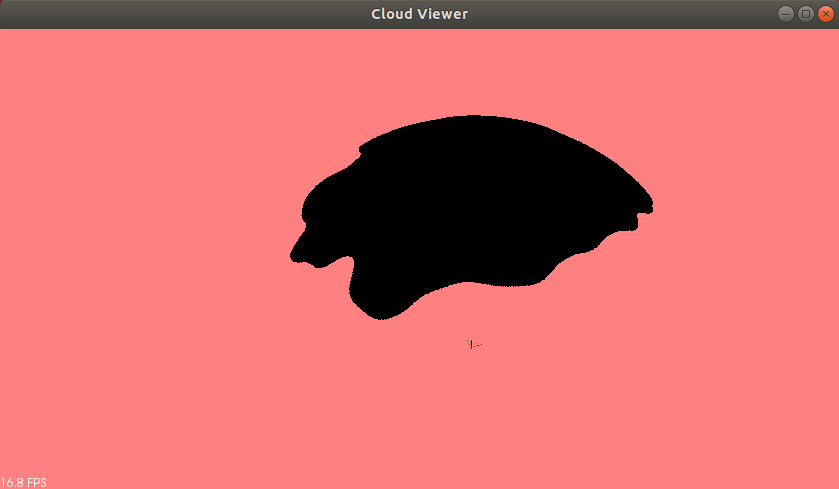
\includegraphics[width=\linewidth]{cturtle_ejemplo}
  \caption{Visualización de la nube $cturtle.pcd$}\label{fig:cturtle_ejemplo}
\endminipage\hfill
\minipage{0.33\textwidth}
  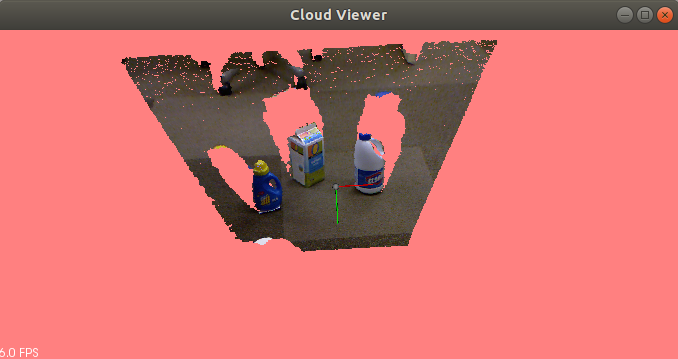
\includegraphics[width=\linewidth]{botes}
  \caption{Visualización de la nube $milk\_cartoon\_all\_small\_clorox.pcd$}\label{fig:botes}
\endminipage\hfill
\end{figure}

\subsection{Extracción de puntos SIFT}
Ahora se quieren extraer los puntos SIFT de estas nubes por lo que se ejecutan los siguientes comandos.
$$./sift\_keypoints\;\;bunny.pcd$$
$$./sift\_keypoints\;\;cturtle.pcd\;\;-mc\;\;0$$
$$./sift\_keypoints\;\;milk\_cartoon\_all\_small\_clorox.pcd$$

Se han utilizado el valor de los parámetros por defecto en $bunny.pcd$ y 
$milk\_cartoon\_all\_small\_clorox.pcd$ pero no ha sido así en $cturtle.pcd$ ya que el parámetro $minimum\_contrast$ tiene un valor de $0$ en vez de $0,001$. Esto se debe a que ninguno de los puntos SIFT detectados supera el filtro de contraste, lo cual parece razonable porque estudiando la superficie que representa $cturtle.pcd$ se ve una curvatura muy suave y a penas tiene bordes y esquinas marcados.

De este modo, el fichero de texto $tests.txt$ generado tras ejecutar estos tres comandos tiene el siguiente contenido:

\begin{lstlisting}
filename: bunny.pcd

Normal estimation radius search: 0.02
Minimum scale: 0.01
Number of octaves: 3
Number of scales per octave: 4
Minimum contrast: 0.001

Normal estimation time (s): 0.034731
SIFT points estimation time (s): 0.040729
Number of SIFT points found: 13
------------------------------
------------------------------
filename: milk_cartoon_all_small_clorox.pcd

Normal estimation radius search: 0.02
Minimum scale: 0.01
Number of octaves: 3
Number of scales per octave: 4
Minimum contrast: 0.001

Normal estimation time (s): 122.083
SIFT points estimation time (s): 5.09761
Number of SIFT points found: 404
------------------------------
------------------------------
filename: cturtle.pcd

Normal estimation radius search: 0.02
Minimum scale: 0.01
Number of octaves: 3
Number of scales per octave: 4
Minimum contrast: 0

Normal estimation time (s): 14.1584
SIFT points estimation time (s): 9.5875
Number of SIFT points found: 952
\end{lstlisting}

Además, cada vez que se extraen los puntos SIFT de una nube, se genera una nube de puntos llamada $sift\_keypoints$ la cual contiene los puntos SIFT de la nube de entrada a este programa. Esto es importante de cara a la siguiente sección de visualización de puntos SIFT.


\subsection{Visualización de puntos SIFT}
Por último, se visualizan en conjunto la nube original y sus puntos SIFT utilizando de nuevo el visualizador el cual se alimenta de dos nubes de puntos: la nube original y la nube $sift\_keypoints$ que contiene sus puntos SIFT y ha sido generada por el programa de extracción de keypoints. En las figuras \ref{fig:botes_ejemplo_sift}, \ref{fig:bunny_ejemplo_sift} y \ref{fig:cturtle_ejemplo_sift} se aprecian los resultados de ejecutar los siguientes comandos:

$$./visualization\;\;bunny.pcd\;\;sift\_keypoints.pcd$$
$$./visualization\;\;milk\_cartoon\_all\_small\_clorox.pcd\;\;sift\_keypoints.pcd$$
$$./visualization\;\;cturtle.pcd\;\;sift\_keypoints.pcd$$


\begin{figure}[!htb]
\minipage{0.32\textwidth}
  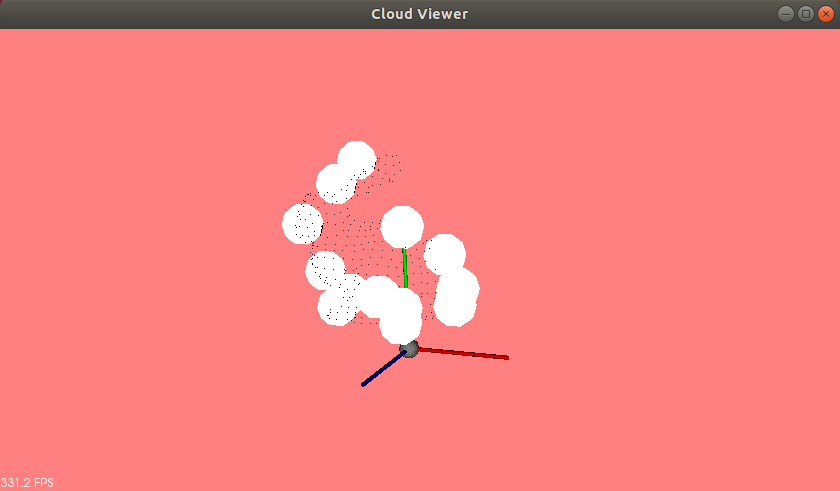
\includegraphics[width=\linewidth]{bunny_ejemplo_sift}
  \caption{Visualización de la nube $bunny.pcd$ junto a sus puntos SIFT como esferas blancas.}\label{fig:bunny_ejemplo_sift}
\endminipage\hfill
\minipage{0.32\textwidth}
  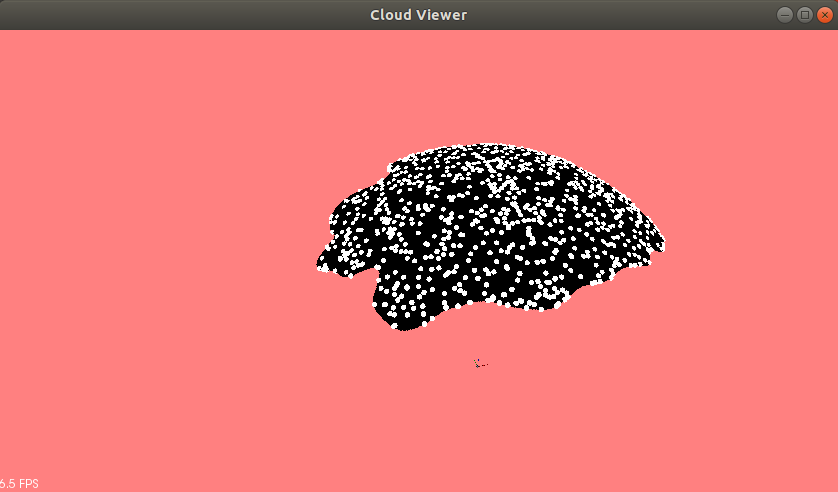
\includegraphics[width=\linewidth]{cturtle_ejemplo_sift}
  \caption{Visualización de la nube $cturtle.pcd$ junto a sus puntos SIFT como esferas blancas.}\label{fig:cturtle_ejemplo_sift}
\endminipage\hfill
\minipage{0.33\textwidth}
  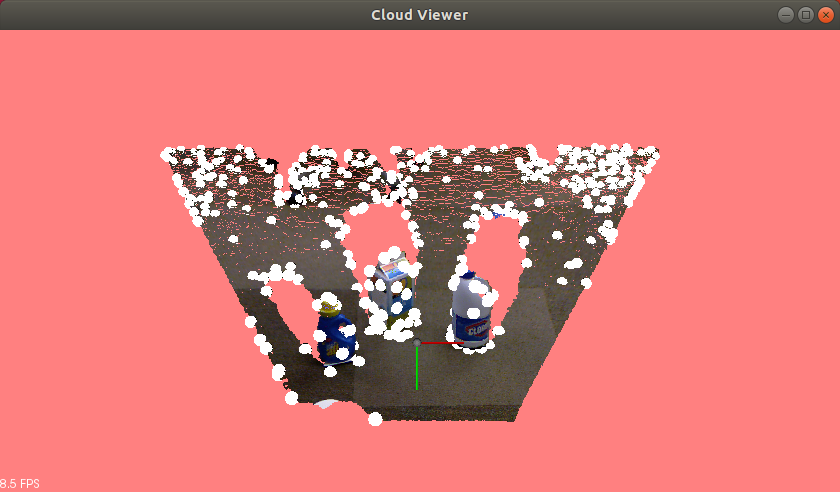
\includegraphics[width=\linewidth]{botes_ejemplo_sift}
  \caption{Visualización de la nube $milk\_cartoon\_all\_small\_clorox.pcd$ junto a sus puntos SIFT como esferas blancas.}\label{fig:botes_ejemplo_sift}
\endminipage\hfill
\end{figure}


\section{Conclusiones}
Se ha visto en este capítulo cómo funcionan dos programas generados a partir de la documentación de PCL para visualizar nubes de puntos y obtener puntos SIFT. Además se ha mostrado su uso en tres nubes de puntos de diferentes características.

En el siguiente capítulo se procederá a medir los tiempos de ejecución de los algoritmos de estimación de vectores normales y puntos SIFT para determinar cuál es el de mayor carga computacional.
